% !TEX program = pdflatex
% Initial submission to the International Journal of Humanoid Robotics.
% The scientific content is inherited from the frozen confirmation analysis.
\documentclass[letterpaper,10pt,conference]{IEEEtran}

\usepackage{amsmath,amssymb}
\usepackage{array}
\usepackage{booktabs}
\usepackage{graphicx}
\usepackage{microtype}
\usepackage[hidelinks]{hyperref}
\graphicspath{{figures/}}
\hypersetup{
  pdftitle={Whole-Body Physics Signatures for Humanoid Gait Failure Ranking},
  pdfauthor={Egor Zharinov},
  pdfsubject={Humanoid gait failure ranking},
  pdfkeywords={humanoid locomotion, whole-body dynamics, failure ranking,
    feasibility screening, reproducible simulation}
}

\newcommand{\talossuccess}{283/400 (70.8\%)}
\newcommand{\icubsuccess}{159/400 (39.8\%)}
\newcommand{\primarydelta}{.034}
\newcommand{\primaryci}{[-.009,.073]}
\newcommand{\bOnePRAUC}{.596}
\newcommand{\bOneROCAUC}{.659}
\newcommand{\bOneTalosPRAUC}{.300}
\newcommand{\bOneICubPRAUC}{.653}
\newcommand{\bTwoPRAUC}{.574}
\newcommand{\bTwoROCAUC}{.655}
\newcommand{\bTwoTalosPRAUC}{.302}
\newcommand{\bTwoICubPRAUC}{.603}
\newcommand{\bThreePRAUC}{.630}
\newcommand{\bThreeROCAUC}{.675}
\newcommand{\bThreeTalosPRAUC}{.273}
\newcommand{\bThreeICubPRAUC}{.694}
\newcommand{\bFourPRAUC}{.689}
\newcommand{\bFourROCAUC}{.763}
\newcommand{\bFourTalosPRAUC}{.495}
\newcommand{\bFourICubPRAUC}{.738}
\newcommand{\bFivePRAUC}{.725}
\newcommand{\bFiveROCAUC}{.770}
\newcommand{\bFiveTalosPRAUC}{.512}
\newcommand{\bFiveICubPRAUC}{.789}

\title{Whole-Body Physics Signatures for Humanoid Gait Failure Ranking}
\author{Egor Zharinov\\
\small Moscow Institute of Physics and Technology (National Research University)\\
\small 9 Institutskiy per., Dolgoprudny, Moscow Region 141701, Russian Federation\\
\small \textit{Corresponding author:}
\href{mailto:egor.zharinov.dev@gmail.com}{egor.zharinov.dev@gmail.com}
\quad ORCID:
\href{https://orcid.org/0009-0005-5362-4460}{0009-0005-5362-4460}}

\begin{document}
\maketitle

\begin{abstract}
Reduced-order checks omit whole-body constraints that can invalidate humanoid
gait candidates. We test whether normalized whole-body physics signatures add
offline failure-ranking information beyond gait parameters and robot identity
on TALOS and iCub. Fixed histogram-based gradient-boosting (HGB) models are fit
on 200 development rollouts and evaluated without refitting on two independent
400-rollout scrambled-Sobol confirmations (seeds 42026 and 52026). The
whole-body model reaches pooled failure PR-AUC/ROC-AUC of
\bFivePRAUC/\bFiveROCAUC{} versus \bFourPRAUC/\bFourROCAUC{} for the fair
parameter-plus-robot comparator. Its prespecified macro within-robot PR-AUC
difference is +\primarydelta{}, with a conditional 95\% bootstrap interval
\primaryci{}. The direction is positive on both scrambles (+.017 and +.032),
but the interval crosses zero, so the confirmatory gate fails. Phase-resolved
and phase-agnostic variants are tied, and a rollout-budget diagnostic shows no
efficiency advantage. The evidence suggests a modest whole-body ranking signal
but does not establish a reliable improvement.
\end{abstract}

\noindent\textbf{Keywords:} humanoid locomotion; whole-body dynamics; failure
ranking; feasibility screening; reproducible simulation

\section{Introduction}
Reduced-order locomotion methods make candidate generation tractable through
preview control, capture-point reasoning, footstep placement, and divergent
components of motion~\cite{kajita2003preview,pratt2006capture,herdt2010online,englsberger2015dcm}.
Their candidates can nevertheless fail once whole-body dynamics, unilateral
contacts, actuator limits, timing error, and impacts are considered. Because
calling a whole-body rollout oracle for every offline candidate is costly, a
preliminary ranking score could reduce the number of required evaluations.
Learning feasibility
constraints~\cite{carpentier2017feasibility} and learning from costly gait
trials~\cite{calandra2016gaits} motivate this direction, but neither line of
work eliminates the need for independent evaluation across robot platforms.

We therefore ask a narrower, directly testable question: after all engineering
choices are frozen, do normalized whole-body physics features add repeatable
failure-ranking information beyond gait parameters and robot identity on new
TALOS~\cite{stasse2017talos} and iCub~\cite{metta2010icub} rollouts? The robots
remain separate evaluation strata; a pooled gain is not interpreted as
morphology transfer.

Our contributions are:
\begin{enumerate}
  \item a normalized whole-body sequence signature evaluated by a separate
  closed-loop rollout oracle;
  \item two independently scrambled 400-rollout confirmations with a frozen
  macro within-robot endpoint; and
  \item a fair robot-aware comparator, representation ablations, and an honest
  negative result when the conditional interval includes zero.
\end{enumerate}

Two 100-row development sets determine the models. Two separate 400-row
confirmation sets are then used once for ranking, conditional bootstrap
inference, and the budget diagnostic; their labels never alter the models or
oracle.

\section{Related Work}
\subsection{Whole-Body Locomotion Feasibility}
Optimization-based locomotion ranges from hierarchical inverse kinematics to
centroidal and multicontact optimal control
~\cite{escande2014hqp,kuindersma2016atlas,winkler2018gait,mastalli2020crocoddyl,ponton2021multicontact}.
Timing adaptation and perceptive nonlinear MPC further show why contacts and
execution timing matter beyond a fixed LIPM plan
~\cite{khadiv2020timing,grandia2023perceptive}. We focus on offline failure
ranking and ask whether inexpensive features derived from a candidate sequence
can rank failures before a separate whole-body rollout.

Carpentier \emph{et al.} learned whole-body kinematic feasibility constraints
for multicontact planning~\cite{carpentier2017feasibility}. Wrench polytopes and
improved feasible regions combine contact, actuation, dynamic-balance, and
kinematic limits~\cite{orsolino2018wrench,abdalla2023feasibility}. Sequence-level
prediction can also reorder costly planning attempts~\cite{yang2023sequence}.
Our contribution lies in the experimental design: the score summarizes an
entire perturbed gait, the label comes from a separate closed-loop rollout, and
the same frozen representation is evaluated on two humanoid models and two
independent scrambles. The contribution is the ranking representation and
evaluation protocol, not a new controller or outer-loop search algorithm.

\subsection{Ranking, Calibration, and Selective Risk}
Ranking metrics characterize discrimination, whereas selective classification
characterizes risk conditional on admission
~\cite{elyaniv2010selective,geifman2019selectivenet}. Probability calibration,
conformal prediction, and risk-controlling prediction offer principled tools
when an independent calibration sample and exchangeability assumptions are
available~\cite{niculescu2005probabilities,guo2017calibration,angelopoulos2023conformal,bates2021rcps}.
Because confirmation has no separate calibration split, we report ranking and
rollout-budget behavior without a calibrated-risk guarantee. Discrimination
alone does not certify selective safety.

\section{Ranking Scores and Frozen Training Data}
\subsection{Sequence Representation and Oracle}
Each six-step candidate is normalized by neutral leg length $L$, neutral width
$w_0$, and $T=\sqrt{L/g}$. Endpoint-$C^2$ foot trajectories are generated with
warm-started bounded manifold inverse kinematics, using manifold integration and
differencing rather than Euclidean quaternion arithmetic. At each reference
state, a two-stage linear program solves for generalized acceleration $a$,
joint effort $\tau$, and world-aligned sole wrenches $\lambda$ subject to
\begin{equation}
 M(q)a+h(q,v)=S^\top\tau+J_c^\top\lambda ,
\end{equation}
rigid-contact acceleration equalities, effort bounds, unilateral normal force,
a friction pyramid, torsional friction, and convex-polygon CoP bounds. The
primary objective minimizes normalized $L_1$ acceleration-tracking slack; at
that optimum, the secondary objective minimizes normalized effort and wrench
magnitude. The LP produces ranking features; it does not define the rollout
label.

For each active sole, the equality
$J_c a+\dot{J}_c v=0$ is imposed in a world-aligned contact frame. With sole
half-length $\ell$, half-width $b$, and wrench
$\lambda=(f_x,f_y,f_z,m_x,m_y,m_z)$, the inequality block includes
\begin{equation}
\begin{aligned}
 f_z&\geq0,& |f_x|,|f_y|&\leq\mu f_z,\\
 |m_x|&\leq b f_z,& |m_y|&\leq\ell f_z ,
\end{aligned}
\end{equation}
plus the torsional bound and effort limits. Slack is attached to desired
acceleration rather than rigid-body consistency, so the dynamics equality
remains auditable. A lexicographic second solve prevents arbitrary large
opposing wrenches among equally good acceleration fits.

Signed channels encode torque, friction, CoP/ZMP, joint-position, and
joint-velocity margins. Nonnegative channels encode IK residual,
acceleration-tracking slack, solver failure, and a touchdown proxy. The
touchdown proxy combines normalized pre-impact contact speed with disturbance
magnitude; it is not an estimated impact impulse. For single support,
touchdown, and double support separately, every channel is aggregated by
minimum, fifth percentile, median, 95th percentile, and maximum. All signature
channels are normalized by robot capacities. For the proposed B5, the three
phase values for each channel/statistic are sorted, preserving their values and
dimension while removing phase identity. The phase-resolved representation is
reported as an ablation rather than claimed as the source of improvement.

Formally, let $c_j(t)$ denote channel $j$ and $\mathcal{I}_p$ the samples in
phase $p$, for $p\in\{\mathrm{SS},\mathrm{TD},\mathrm{DS}\}$. Using
$\mathcal{A}=\{\min,Q_{.05},Q_{.50},Q_{.95},\max\}$, the signature is
\begin{equation}
 \phi=\left[\;a\!\left(\{c_j(t):t\in\mathcal{I}_p\}\right)\;\right]_{
 p,j,a\in\mathcal{A}} .
\end{equation}
Ten channels, three phases, and five aggregations yield 150 values. Appending
the eleven gait/disturbance parameters and one binary robot indicator gives B5
a 162-dimensional input; B4 receives the same parameters and robot indicator.
Thus their difference isolates summarized whole-body physics rather than
classifier capacity or unequal access to robot identity.

A separate closed-loop whole-body rollout oracle, implemented in
Pinocchio~\cite{carpentier2019pinocchio}, provides labels for both robots.
Continuous single/double support uses constrained rigid-body dynamics;
touchdown first tests admissible perfectly inelastic sticking-contact subsets
and otherwise falls back to a unilateral vertex-contact solve. Feed-forward
inverse dynamics plus normalized PD feedback controls the nominal model.
Payload changes only the torso inertia in the plant model, while friction
variation, timing error, and a seeded horizontal impulse perturb execution. The
labels therefore reflect
closed-loop model mismatch rather than a second evaluation of the reference
generator.

With $\omega=\sqrt{g/L}$, the controller requests
\begin{equation}
 a_d=a_{\rm ref}+20\omega^2\operatorname{difference}(q,q_{\rm ref})
       +8\omega(v_{\rm ref}-v).
\end{equation}
Inverse dynamics maps $a_d$ to feed-forward-plus-feedback effort under the
realized contact set. We log unconstrained demand, then resolve with URDF effort
limits when demand saturates. The plant integrates the resulting constrained
acceleration on the configuration manifold. At touchdown, admissible sticking
subsets are tested with impulse dynamics; an infeasible full-sole impact may
drop to unilateral vertex contacts rather than being accepted by construction.

The first-failure categories are normal-force, friction, CoP, joint
position/velocity, collision, fall, tracking, and dynamics.
Contact failure is evaluated from realized rollout wrenches, not a reduced-order
ZMP formula. A rollout also fails if pelvis height falls below 65\% of neutral,
roll/pitch exceeds $30^\circ$, CoM error exceeds $0.12L$, or contact/impact
dynamics cannot be solved. Applied torque is saturated at URDF limits; the
unsaturated demand is diagnostic rather than a failure label. Joint position or
velocity must exceed the corresponding limit by more than 1\% for at least
20~ms. These rigid-contact mechanics and numerical transition tolerances are
evaluation choices, not a physical safety certificate.

The signature and label deliberately use different information. Signature
channels are computed along the planned whole-body reference by the
inverse-dynamics LP. The rollout begins from that reference but evolves a
payload-perturbed plant under saturated feedback, realized contact transitions,
and a seeded impulse. Consequently, a large signature margin may coexist with
a failed rollout, and B5 must learn associations rather than reproduce an
oracle rule. This separation prevents target leakage from realized failure
times or rollout wrenches into the ranking features.

\subsection{Normalization and Oracle Validity}
Geometric inputs use robot-specific physical capacities. Lengths are divided by
$L$ or the relevant sole half-dimension,
durations by $T$, forces by $mg$, joint efforts by URDF effort limits, and
external impulse by $m\sqrt{gL}$. The neutral width $w_0$ is the lateral
distance between sole centers. Sole support polygons are the convex hulls of
the lowest vertices in the manually reviewed, axis-normalized collision meshes.
This design aims to make equivalent margins comparable. Both learned scores
also receive the same binary robot indicator so the comparator is not denied
base-rate information available implicitly in physical features.

Several numerical guards prevent transition artifacts from causing failures.
The CoP moment inequality includes both a $10^{-4}L$ geometric tolerance and an
absolute force-tolerance floor, so a nearly unloaded contact is not divided by
an arbitrarily small normal force. Flat-terrain penetration has a
$10^{-3}L$ continuous limit and a $2\times10^{-3}L$ hard transition bound.
Within that band, contact state, vertical velocity, and one-step predicted gap
determine whether the event is recovery, liftoff, or reimpact. Scheduled and
realized contacts are logged separately; the oracle does not force a planned
double-support phase to remain active.

Before confirmation, the unchanged oracle passed the repository's
analytic validity suite: valid manifold configurations and unit quaternions,
normalized rigid-body residual below $10^{-6}$, reviewed wrench/CoP signs and
frames, a feasible static double-support pose, and correct rejection of injected
torque, friction, collision, and impact failures. No oracle parameters were
changed for the evaluation. Each case is simulated at 100~Hz and written
atomically before aggregate statistics are updated.

\subsection{Five Fixed Ranking Scores}
The two development sets contain 200 labeled rollouts, exactly 100 per robot.
They include all oracle and representation engineering; they are used to freeze
the proposed representation and fit B4/B5. The HGB configuration uses a
maximum of seven leaf nodes, learning rate
0.08, 150 iterations, $\ell_2$ regularization 1.0, and random state 2026; there
is no tuning, threshold selection, recalibration, or refitting with confirmation
outcomes. We compare five scores:
\begin{description}
  \item[B1] ZMP/CoP margin;
  \item[B2] IK and joint-limit margin;
  \item[B3] worst phase-aggregated dynamics slack;
  \item[B4] HGB using gait/perturbation parameters and robot identity; and
  \item[B5] HGB using the same inputs plus the normalized, phase-agnostic
  whole-body signature.
\end{description}
For all scores, a larger value means a higher predicted likelihood of oracle
failure. The physics baselines are deliberately simple. Giving the same robot
indicator to B4 and B5 prevents morphology-dependent failure prevalence from
being credited only to B5. HGB is a standard compact nonlinear baseline
~\cite{friedman2001boosting}.

\section{Independent Confirmation Protocol}
The revised endpoint and code were frozen before evaluation (commit
\texttt{88c1b41}). An earlier seed-32026 set informed this revision and is
excluded from all results below. Confirmations use seeds 42026 and 52026, each
with 400 new six-step rollouts (200 per robot). Every rollout seed is disjoint
from development and from the other confirmation. The frozen common domain is
step length $[0.10,0.16]L$, width $[1.00,1.10]w_0$, single-support duration
$[2.70,2.80]T$, double-support duration $[0.70,0.80]T$, CoM-height scale
$[0.92,0.98]$, ZMP biases $x\in[-0.05,0.05]$ and
$y\in[-0.25,-0.10]$, friction $[0.4,0.8]$, payload $[0,0.05]m$, timing error
$[-0.02,0.02]$~s, and normalized horizontal impulse $[0,0.04]$. Gait and
perturbation marginals use separately scrambled Sobol streams with a
deterministic pairing.

\begin{table}[t]
\caption{Frozen Data Roles}
\label{tab:data}
\centering
\footnotesize
\setlength{\tabcolsep}{2.6pt}
\begin{tabular}{@{}lcccc@{}}
\toprule
Set & Seed & Samples/robot & Payload & Label use \\
\midrule
Development A & 12026 & 50  & $[0,.10]m$ & engineer/fit \\
Development B & 22026 & 50  & $[0,.05]m$ & select/fit \\
Confirmation A & 42026 & 200 & $[0,.05]m$ & test once \\
Confirmation B & 52026 & 200 & $[0,.05]m$ & test once \\
\bottomrule
\end{tabular}
\end{table}

The primary endpoint is the macro within-robot difference
\begin{equation}
D=\frac{1}{2}\sum_{r\in\{\mathrm{TALOS,iCub}\}}
\left[\operatorname{AP}_r(\mathrm{B5})-\operatorname{AP}_r(\mathrm{B4})\right],
\end{equation}
where PR-AUC treats failure as positive. We draw 10,000 paired bootstrap
samples within each $(\text{scramble},\text{robot})$ stratum. The gate requires
a positive percentile-CI lower endpoint and a positive point difference on
each scramble. Confirmation labels cannot alter the oracle, domain,
representation, models, hyperparameters, or seeds.

Scores are predicted once and held fixed across resamples. Because the rows
come from two scrambled quasi-random designs rather than IID sampling, the
interval is explicitly conditional and descriptive, not a nominal population
coverage guarantee. Pairing compares B4/B5 on identical cases; the two
independent scrambles directly expose sign stability.

As a descriptive deployment diagnostic, 10,000 deterministic pools of 50
confirmation candidates per robot are sampled without replacement. B4 and B5
rank the same pool from lowest predicted failure probability upward; we record
success within budgets $\{5,10,20\}$ and the rank of the first feasible gait.
The artifact verifies row counts, seed disjointness, source/protocol
fingerprints, and SHA-256 hashes before analysis.

\section{Confirmation Results}
The frozen oracle returns \talossuccess{} successful TALOS rollouts and
\icubsuccess{} successful iCub rollouts. TALOS has 107 friction, seven
normal-force, two tracking, and one impact-dynamics failure; iCub has 109
friction, 106 normal-force, ten impact-dynamics, eight tracking, seven
collision, and one CoP failure. Mean oracle runtimes are 13.30~s and 9.94~s,
respectively. The different base rates motivate within-robot inference.

We report PR-AUC because failure prevalence differs, with ROC-AUC as a
complementary ranking metric~\cite{saito2015precision}. Table~\ref{tab:ranking}
contains confirmation-only results.

\begin{table}[t]
\caption{Confirmation Failure-Ranking Metrics}
\label{tab:ranking}
\centering
\footnotesize
\setlength{\tabcolsep}{2.4pt}
\begin{tabular}{@{}lcccc@{}}
\toprule
Score & PR-AUC & ROC-AUC & TALOS PR & iCub PR \\
\midrule
B1 ZMP/CoP       & \bOnePRAUC & \bOneROCAUC & \bOneTalosPRAUC & \bOneICubPRAUC \\
B2 IK/joint      & \bTwoPRAUC & \bTwoROCAUC & \bTwoTalosPRAUC & \bTwoICubPRAUC \\
B3 slack         & \bThreePRAUC & \bThreeROCAUC & \bThreeTalosPRAUC & \bThreeICubPRAUC \\
B4 parameters+ID & \bFourPRAUC & \bFourROCAUC & \bFourTalosPRAUC & \bFourICubPRAUC \\
B5 whole-body    & \bFivePRAUC & \bFiveROCAUC & \bFiveTalosPRAUC & \bFiveICubPRAUC \\
\bottomrule
\end{tabular}
\end{table}

\begin{figure}[t]
  \centering
  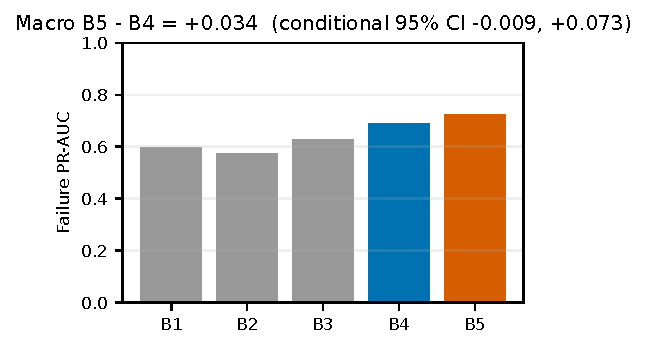
\includegraphics[width=\columnwidth]{figure2_domain_gate.pdf}
  \caption{Confirmation PR-AUC. The prespecified macro within-robot B5--B4
  difference is positive, but its conditional bootstrap CI includes zero.}
  \label{fig:ranking}
\end{figure}

B5 reaches pooled PR-AUC/ROC-AUC \bFivePRAUC/\bFiveROCAUC{} versus
\bFourPRAUC/\bFourROCAUC{} for the fair B4 comparator. The macro within-robot
difference is +\primarydelta{} with conditional 95\% CI \primaryci{}
(Fig.~\ref{fig:ranking}). Point differences are positive on both independent
scrambles (+.017 and +.032), but the interval crosses zero; the prespecified
gate therefore fails. Combined per-robot gains are modest on TALOS
(.512 versus .495) and larger on iCub (.789 versus .738). Relative to the
strongest simple margin B3, B5 adds .095 pooled PR-AUC, but this secondary
point comparison has no confirmatory interval.

\subsection{Representation and Rollout Budget}
Table~\ref{tab:ablations} tests the central representation choices.
Phase-resolved and phase-agnostic variants are effectively tied
(.727 versus .725 pooled PR-AUC); removing touchdown features gives .712.
Thus the experiment does not support a benefit from phase identity.

\begin{table}[t]
\caption{Confirmation Representation Ablation}
\label{tab:ablations}
\centering
\scriptsize
\setlength{\tabcolsep}{2.2pt}
\begin{tabular}{@{}lccc@{}}
\toprule
Representation & Pooled PR/ROC & TALOS PR/ROC & iCub PR/ROC \\
\midrule
Phase-agnostic (B5) & .725/.770 & .512/.708 & .789/.736 \\
Phase-resolved      & .727/.772 & .522/.720 & .790/.734 \\
No touchdown        & .712/.770 & .536/.718 & .765/.715 \\
\bottomrule
\end{tabular}
\end{table}

At budget five, both scores find a feasible gait in at least 99.89\% of
50-candidate pools; all budget-10 and budget-20 trials succeed. Mean ranks to
the first feasible gait are 1.000 (B4) versus 1.011 (B5) for TALOS and 1.074
versus 1.319 for iCub (Fig.~\ref{fig:budget}). Thus the whole-body score does
not reduce rollout cost in this high-coverage domain.

\begin{figure*}[t]
  \centering
  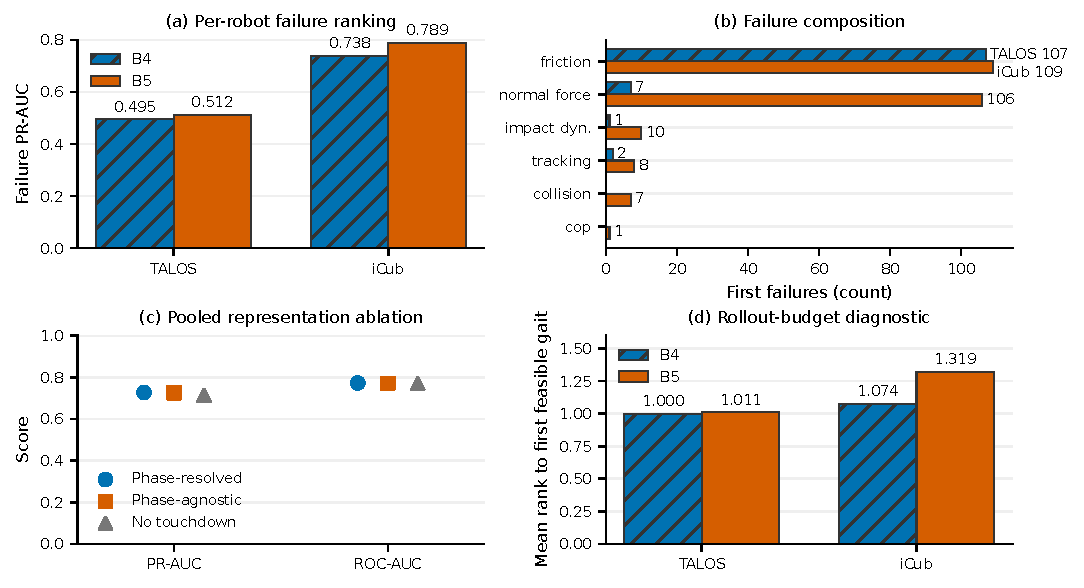
\includegraphics[width=0.98\textwidth]{figure3_heldout_ranking.pdf}
  \vspace{-1mm}
  \caption{Repeated-confirmation summary. (a) B5 has a small positive PR-AUC
  point difference on both robots. (b) First-failure composition differs by
  robot. (c) Phase-resolved and phase-agnostic variants are tied.
  (d) B5 yields no rollout-budget advantage (lower is better).}
  \label{fig:budget}
\end{figure*}

\section{Discussion}
The repeated confirmation gives a deliberately narrower result than the
exploratory analysis. Whole-body features show the same positive point
direction on two new scrambles, but the macro effect is small and its
conditional interval includes zero. The evidence therefore suggests additional
ranking information but does not establish a reliable improvement over a fair
parameter-plus-robot comparator. The larger iCub gain and small TALOS gain also
show that one pooled number should not be read as morphology invariance.

Phase identity is not supported: phase-resolved and phase-agnostic
representations are tied, while touchdown removal is mildly worse only in
pooled data. Feasible candidates are also common enough that both learned
scores almost always succeed within five rollouts; improved discrimination
does not imply lower search cost in this domain.

The apparent tension is expected. PR-AUC measures ordering over all failures,
including difficult cases deep in the list. Search success at a small budget
depends only on whether at least one of the first few candidates is feasible.
With 70.8\% TALOS and 39.8\% iCub feasibility, that event saturates even when
the detailed failure ordering improves. These metrics answer different
questions and should not be substituted for one another.

For use, the workflow is therefore score, shortlist, then verify every selected
candidate with the full oracle. A shared acceptance rule would require new
calibration data and a prespecified risk-control procedure. The score is a
ranking aid, not a safety filter.

\section{Reproducibility and Limitations}
Supplementary Artifact S1 archives both development CSVs, all 800 confirmation
records from two scrambles, source/environment fingerprints, validity reports,
fixed analysis, and figures. Supplementary Video V1 shows successful and failed
rollouts for both robots. One command refits B4/B5, verifies hashes and seed
disjointness, and recreates the reported JSON and figures. Robot meshes are not
redistributed. The same code and data are available in the public
repository~\cite{zharinov2026repository}.

Without a calibration split, the study cannot evaluate 5\% risk control via a
selective threshold or Clopper--Pearson bound, or make an exchangeability-based
guarantee. The budget analysis reuses confirmation candidates and is
descriptive. All labels come from one simulator stack, and the rigid-contact
oracle is not a physical safety certificate. The scope is two simulated
morphologies on flat ground, six-step near-neutral references, one controller,
and one reviewed oracle. Compliance, state estimation, latency, thermal
effects, hardware contacts, and leave-one-morphology-out transfer remain
outside the evidence.

\section{Conclusion}
Across 800 untouched TALOS/iCub rollouts in two independent scrambles, the
whole-body model reaches .725 pooled PR-AUC versus .689 for a fair
parameter-plus-robot comparator. The macro within-robot difference is
+\primarydelta{} with conditional 95\% CI \primaryci{}: positive on both
scrambles, but inconclusive because the interval crosses zero. Phase identity
and rollout-budget savings are not supported. The result is an honest
simulation benchmark, not evidence of calibrated risk control, transfer, or
safety.

\section*{Funding}
This research did not receive any specific grant from funding agencies in the
public, commercial, or not-for-profit sectors.

\section*{Declaration of Competing Interest}
The author declares that he has no known competing financial interests or
personal relationships that could have appeared to influence the work reported
in this paper.

\section*{Data and Code Availability}
The development and confirmation records, analysis and figure-generation code,
environment and source fingerprints, validity reports, and rollout video are
available in Supplementary Artifact S1 and the public repository
\cite{zharinov2026repository}.

\section*{CRediT Authorship Contribution Statement}
Egor Zharinov: Conceptualization, Methodology, Software, Validation, Formal
analysis, Investigation, Data curation, Writing---original draft,
Writing---review and editing, Visualization.

\section*{Use of Generative AI}
OpenAI Codex assisted with research-code implementation, review, and language
clarity. The author verified all outputs and takes full responsibility for the
article.

\IEEEtriggeratref{19}
\bibliographystyle{IEEEtran}
\bibliography{references}
\end{document}
